
\chapter{Evaluation}\label{ch:evaluation}

This section evaluates the performance gained by implementing the logic for dynamically tracking information flow in JIT-compiled code.
The techniques used to validate that the implemented logic correctly tracks the flow of information also deserve emphasis.
Finally, we distinguish the limitations that arise as implementation artifacts from the fundamental limitations of the information flow approach.

WebKit contains an interpreter, JavaScriptCore (JSC), that executes a bytecode instruction sequence using direct threaded interpretation\footnote{
In March 2012, JavaScriptCore changed to a low-level interpreter, implemented via a custom language that generates the assembly for a direct threaded interpreter.
The benchmarks shown here measure the performance of the C++ version of JSC that predates this change.
}.
The WebKit project also contains a template JIT compiler that compiles the bytecode instruction stream and an optimizing JIT compiler based on a program's data-flow graph.
\JitFlow\ builds upon the template JIT and does not implement information flow in the optimizing version of the JIT compiler, because it operates only on Macintosh operating systems.
All of the following benchmarks compare information flow implementations of interpreter-only and JIT-only execution modes.

\begin{table}[ht]
\centering
\resizebox{\columnwidth}{!}{
\begin{tabular}{r l l l}
\textit{Overhead} & \textit{Language} (implementation) & \textit{Reference}                & \textit{Benchmarks}\\
\toprule
80\%              & JS Interpreter (64~bit labels)     & Kerschbaumer~et~al.~\cite{kerschbaumer.etal+13} & SunSpider\\
100 -- 200\%      & JS Interpreter (64~bit labels)     & Just~et~al.~\cite{just.etal+11}         & V8\\
110 -- 690\%      & JS (rewriting during parse)        & Jang~et~al.~\cite{jang.etal+10}         & meas. by visiting pages\\
120\%             & JS Interpreter (data-flow only)    & Tran~et~al.~\cite{tran.etal+12}         & SunSpider\\
136 -- 560\%      & JS Interpreter (only tags objects) & Dhawan and Ganapathy~\cite{dhawan.ganapath+09}   & SunSpider, V8\\
$\sim$200\%       & JS Interpreter (multi-execution)   & Groef~et~al.~\cite{groef.etal+12}        & V8\\
none reported     & JS Interpreter (1~bit label)       & Vogt~et~al.~\cite{vogt.etal+07}         & no perf numbers given\\

14\%              & Java (data-flow only)              & Enck~et~al.~\cite{enck.etal+10}         & CaffeineMark\\
200\%             & Java (JikesRVM)                    & Chandra~and~Franz~\cite{chandra.franz+07}     & JavaGrande \\

1.6\% -- 26.7\%   & C (instrumenting compiler)         & Nanda~et~al.~\cite{nanda.etal+07}        & LAMP-stack\\
24\% -- 1,120\%   & C (instrumenting compiler)         & Lam~and~Chiueh~\cite{lam.chiueh+06}        & C-Programs\\
1,900\%           & x86 VM                             & Yin~et~al.\cite{yin.etal+07}          & CPU Instruction level tainting\\
\bottomrule
\end{tabular}
}
\caption{Performance Comparison of other Information Flow Frameworks}
\label{tab:jitflow-perfcomparison}
\end{table}

%------------------------------------------------------------------------------------------------------
\subsection{Effect on Performance}
\label{ch:evaluation-sec:jitflow-performance}

To demonstrate how JIT compilation of dynamic information flow tracking reduces the performance impact within an information-flow tracking VM, we execute three established JavaScript benchmark suites:
SunSpider version 1.0~\cite{sunspider}, V8 version~6~\cite{v8}, and Kraken version 1.1~\cite{kraken}.
A dual Quad Core Intel Xeon E5462 2.80~GHz with 9.8~GB RAM running Ubuntu~11.10 (kernel 3.2.0) executes all benchmarks using \texttt{nice~-n~-20} to minimize operating system scheduler effects.
After running each suite once for warm-up, the test software executes 10 repetitions for each benchmark to obtain stable results and reports the geometric mean of these repetitions to discount outliers.
Note that the results for these benchmarks do not include the overhead for JIT compiling the code since this happens during the warm-up run.

Previous implementations of information flow (\autoref{tab:jitflow-perfcomparison}) experience a handicap by beginning with an unmodified interpreter that performs an average of 287\% slower than JIT-compiled code.
On a relative basis, \JitFlow\ outperforms all of the previous work listed in \autoref{tab:jitflow-perfcomparison}.
\JitFlow\ also outperforms on an absolute basis when measured with respect to much faster JIT-compiled code.

\begin{figure}[ht]
  \centerline{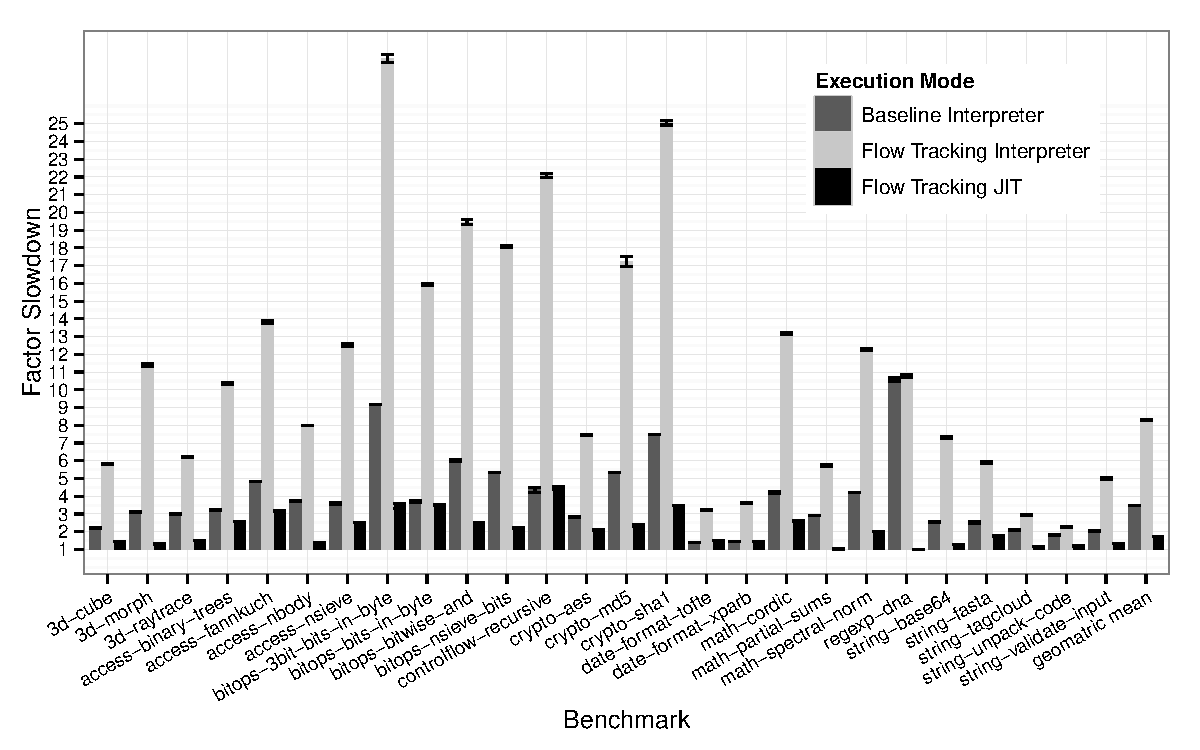
\includegraphics[width=\linewidth,keepaspectratio=true]{graphics/sunspider_plot.pdf}}
  \caption{Detailed performance for the SunSpider benchmark normalized by the \code{JavaScriptCore} JIT compiler.}
   \label{fig:sunspider-performance}
\end{figure}

\begin{figure}[ht]
  \centerline{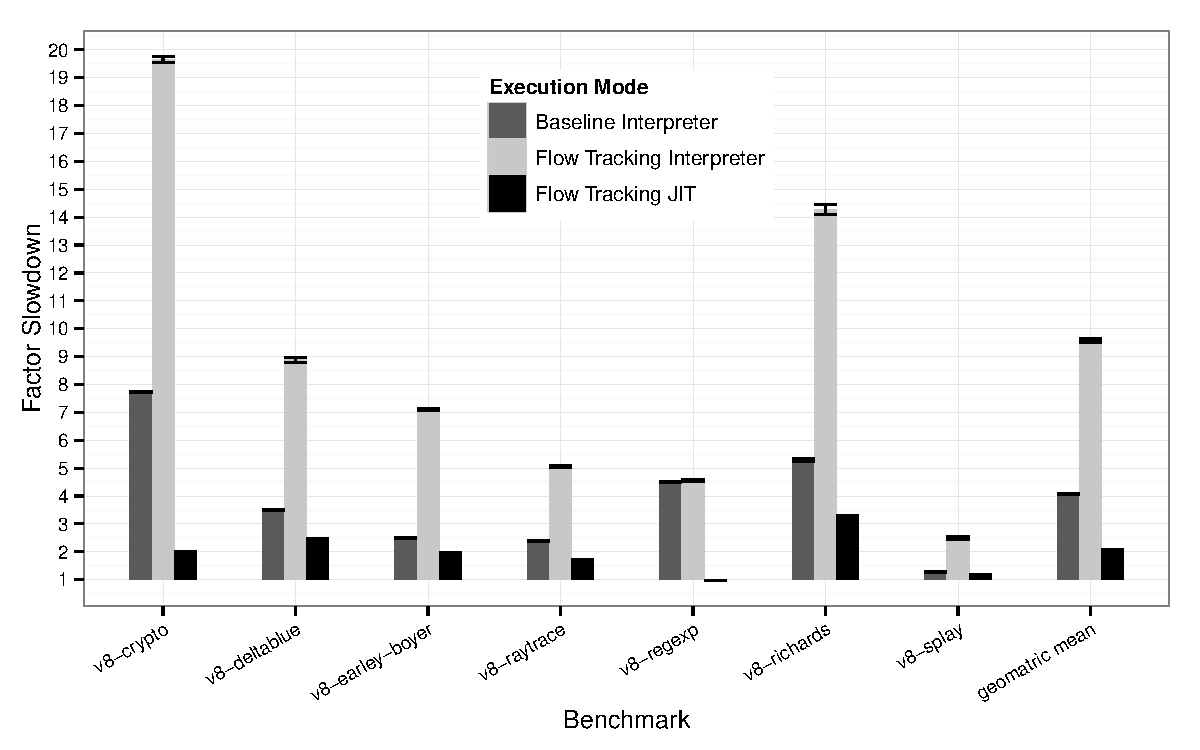
\includegraphics[width=\linewidth,keepaspectratio=true]{graphics/v8_plot.pdf}}
  \caption{Detailed performance for the V8 benchmark normalized by the \code{JavaScriptCore} JIT compiler.}
   \label{fig:v8-performance}
\end{figure}

\begin{figure}[ht]
  \centerline{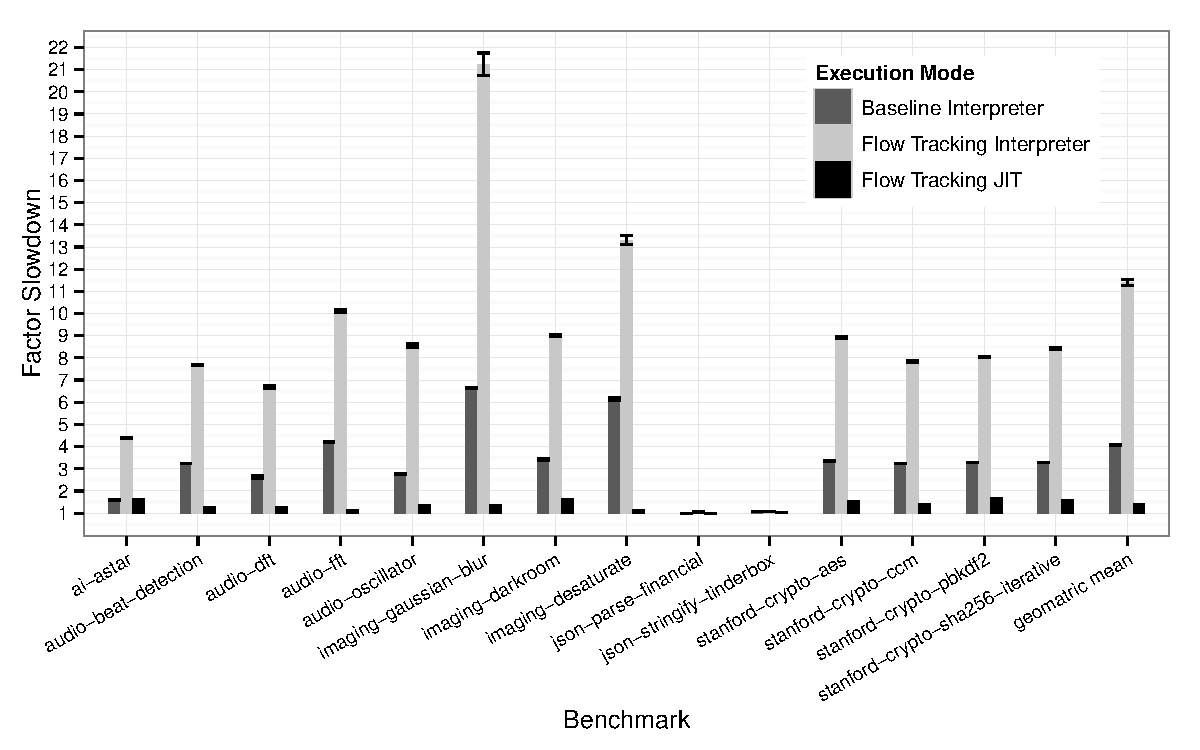
\includegraphics[width=\linewidth,keepaspectratio=true]{graphics/kraken_plot.pdf}}
  \caption{Detailed performance for the Kraken benchmark normalized by the \code{JavaScriptCore} JIT compiler.}
   \label{fig:kraken-performance}
\end{figure}

To provide a consistent basis for performance comparison, we implemented information flow tracking in WebKit's interpreter and JIT compiler using the same label encoding and supporting data structures introduced in \autoref{ch:label-propagation}.
%The comparison required creating a 32-bit version of \FlowCore\ that implements inline labels, rather than the fat values discussed previously.
The benchmarks measure the performance of JIT-compiled tracking code (\JitFlow) vs. interpreter code (\FlowCore) in exclusive modes.
As illustrated in Figures~\ref{fig:sunspider-performance}, \ref{fig:v8-performance}, and \ref{fig:kraken-performance}, the average performance impact for \JitFlow\ (Sunspider~74\%, V8~108\%, and Kraken~38\%) clearly demonstrates that JIT-compiled code implementing dynamic information flow tracking outperforms the execution speed of an unmodified interpreter.
Hence, the \JitFlow\ implementation sets a new bar for dynamic information flow systems.

At the outset, we engineered and incorporated the information flow tracking logic in the JavaScriptCore interpreter, creating \FlowCore.
This effort gave us a deep understanding of WebKit's JavaScript VM and allows a comparison between the relative performance impacts of implementing dynamic information flow tracking in the interpreter vs. the JIT compiler.
Even when implementing information flow in a JIT compiler, the overhead measured as percentage relative to the baseline does not necessarily correspond to that seen when implementing the same framework within the JavaScript interpreter.
For example, the SunSpider benchmark (\autoref{fig:sunspider-performance}) shows an overhead of 137\% in the interpreter, while the JIT compiler shows only 74\%.
\autoref{ch:benchmarks} contains a full account of the performance on each individual benchmark (using the encoding and framework as described in \autoref{sec:jitflow-labelencoding}).

Many of the benchmarks, such as \code{regexp} in V8 and the \code{json} family of tests in Kraken, run with essentially the same speed as the unmodified JIT compiler.
These tests perform fewer control-flow branches and make a higher percentage of native code calls compared to other tests.
Meanwhile, the \code{controlflow-recursive} test in SunSpider introduces the most overhead, at 346\%, because it has a very large number of executed branches in recursive function calls and conditional tests.
These control-flow constructs cause the dynamic information flow VM to perform additional work to maintain the control-flow stack.
Each time the VM recursively calls a function, branches on a conditional, or iterates a loop, it executes the control-flow tracking instructions (\autoref{ch:implementation-sec:instructions}), incurring an overhead relative to an unmodified VM.

Overall, the low impact for the JIT-compiled information flow tracking logic (73\% on average, on compute intensive benchmarks) highlights the practicality of dynamic information flow as a security enhancement for the outdated JavaScript security model.

\subsubsection{Impact of Conservatively Labeling Doubles}
\label{sec:jitflow-impact-doubles}

As previously stated in \autoref{sec:jitflow-labelencoding}, the current format of doubles within WebKit does not allow directly encoding a label within the representation of a double.
All operations involving doubles implicitly carry the highest label available at the time they execute.
This conservative labeling strategy might conceal the performance drawback for benchmarks focusing on doubles.

To show that this implementation detail has little performance impact, we report the percentage of operations creating doubles vs. other \jsvalues\ for each of the three benchmark suites.
In SunSpider, doubles comprise 4.7\% of created \jsvalues\, while in the other test frameworks double comprise fewer than 1\%, 0.23\% in V8, and 0.96\% in Kraken.
This ratio lets us conclude that, in those three benchmark suites, doubles account for only a small fragment of created values and therefore do not influence the overall performance impact.

\subsection{Correctness}
\label{sec:jitflow-evaluation-correctness}

The \JitFlow\ implementation, including \FlowLabelRegistry\ and other data structures, adds approximately 4,000 lines of C++/assembly code to WebKit's codebase\footnote{Calculated by performing a \texttt{git diff base | grep "\textasciicircum+[\textasciicircum+]" | wc -l}}.
To validate that the modifications \JitFlow\ makes to JavaScriptCore's JIT engine for tracking the flow of information throughout execution of a JavaScript program do not introduce any errors, we made sure that none of our modifications broke any of the Mozilla regression tests in the WebKit repository.
This suite consists of over 1,000 test cases covering core JavaScript functionality, including arrays, dates, functions, numbers, objects, regular expressions, and strings.

In addition, we wrote a suite of test cases that check the correct label propagation for the information flow tracking logic and added them to the regression suite.
These tests exercise label propagation for all of the implemented binary operations and control-flow structures: \code{if}-statements, the various loop constructs including break and continue statements, \code{eval}, and function calls.
These these tests make use of a first-class labeling framework~\cite{hennigan.etal+13} (\autoref{ch:first-class-labels}) that permits explicit application and inspection of labels within the JavaScript language itself, allowing incorporation of the test cases into the regression suite.

\lstset{
  caption={Regression test verifying correct label propagation for additions.},
  label={list:jitflow-regressiontest},
}
\begin{jscode}
var a = (new FlowLabel("labelA"))(24);
var b = (new FlowLabel("labelB"))(12);

var res = a + b;

reportCompare(36, res, "add value incorrect.");
reportCompare(true, (labelof res).subsumes(labelof a),
              "wrong first label in add");
reportCompare(true, (labelof res).subsumes(labelof b),
              "wrong second label in add");

reportCompare((labelof res), (labelof a).join(labelof b),
              "wrong joined label in add");
\end{jscode}

\autoref{list:jitflow-regressiontest} shows one of the crafted regression tests for confirming correct label propagation.
In keeping with the other examples (\autoref{ch:implementation-sec:jitflow-tracking-data-flow}), this test focuses on the correct label propagation for integer addition.

The integer addition test begins by giving each of the input operands separate labels.
\Codeline{1} assigns input variable \code{a} the value \code{24} with label \code{labelA} (internally mapped to \code{0001}) and \codeline{2} assigns input variable \code{b} the value \code{12} with label \code{labelB} (internally mapped to \code{0010}).

After initialization, the test performs the addition on \codeline{4}.
To provide feedback during development, the test uses the \code{reportCompare} function, provided by the regression suite.
On \codeline{6}, it checks that the result has value \code{36} as expected.

Further sanity checking occurs on \codelines{7}{10} to ensure that the label attached to the result subsumes the label attached to each of the inputs.
Finally, on \codeline{12}, the test verifies that the label attached to the result of the addition (\code{0011}) matches the join of the labels on the operands (\code{0001|0010}).

%------------------------------------------------------------------------------------------------------
\subsection{Real World Applicability}
\label{sec:realworldapplicability}

Conforming to the capabilities of the attacker (\autoref{sec:defense-attackers-threat}), this evaluation defines an information flow violation as the inequality of domains between a network data payload and the target.
When the label of the payload indicates that the data has been influenced by any origin other than the destination domain, the network request represents a communication to a foreign party, possibly an attacker-controlled server.

To verify that \JitFlow\ detects information flow violations, a web crawler automatically visits web pages and stays on each web page for 60~seconds.
The web crawler visits a randomly sampled selection 100 of the Alexa~Top~one~million~\cite{alexa} web pages.
To simulate user interaction, the web crawler fills out HTML-forms and submits the first available form on each visited page.
For all of the following results, the crawler used information flow in both the JIT compiler and the interpreter, demonstrating a seamless switch between the two, as occurs in real-world browsing.

\begin{table*}[ht!]
\centering
\resizebox{\columnwidth}{!}{
\begin{tabular}{r|r|l|r || r|l|r}
& \multicolumn{3}{c||}{Ranked by Number of Included Domains} & \multicolumn{3}{c}{Ranked by Number of Flow violations} \\
 & \textit{Alexa Rank} & \textit{Page} & \textit{Dom.}  & \textit{Alexa Rank} & \textit{Page} & \textit{Flows}\\
\hline
1 & 556,895 & \url{prizyvnikmoy.ru} & 13 & 683,716 & \url{onefeat.com} & 295 \\
2 & 540,606 & \url{finn-dinghy.de} & 13 & 592,642 & \url{train-shop.net} & 80 \\\
3 & 438,078 & \url{mitula.ch} & 13 & 196,697 & \url{nudepornstarz.net} & 78 \\
4 & 19,658 & \url{roxio.com} & 13 & 394,557 & \url{just-eat.no} & 51 \\
5 & 999,112 & \url{printertransferroller.blogspot.com} & 12 & 889,993 & \url{sfee.gr} & 49 \\
6 & 799,519 & \url{masteringonlinemarketing.com} & 12 & 801,235 & \url{aksgonline.com} & 37 \\
7 & 683,716 & \url{onefeat.com} & 12 & 556,895 & \url{prizyvnikmoy.ru} & 35 \\
8 & 507,796 & \url{ifm-bonn.org} & 12 & 992,317 & \url{mentoring-uk.org.uk} & 30 \\
9 & 494,397 & \url{natives.co.uk} & 12 & 540,774 & \url{buildinglebow.com} & 27 \\
10 & 472,505 & \url{wcode.ru} & 12 & 834,020 & \url{tct.net.ua} & 24 \\
\hline
& & Average (of all 100 pages)& 7 & & Average (of all 100 pages)& 12 \\
\end{tabular}
}
\caption{Web pages including content from the greatest number of different domains (left) and web pages having the greatest number information flow violations (right).}
\label{tab:webstatistics}
\end{table*}

\subsubsection{Including other domains.}

Modern web applications integrate content from several different origins on the web.
The collected statistics show that each of the visited web pages include an average of 7~different origins for their content.
The inline label approach lets \JitFlow\ directly encode up to 16 different domains within one label.
This technique permits an efficient encoding even for the web pages including the most content: \url{prizyvnikmoy.ru}, \url{finn-dinghy.de},  \url{mitula.ch}, and \url{roxio.com} including content from 13 domains.
These findings complement the results of Nikiforakis et al~\cite{nikiforakis.etal+12}, who visited over three million pages for their empirical study showing that more than 90\% of all pages include code from less than 15 different domains.

\subsubsection{Information flow violations}

The \JitFlow\ web crawler first visited the sample of pages using the interpreter and found 1,155 information flow violations.
The page \url{onefeat.com} had the highest observed number of violating flows, at 295.
On average, the crawler detected 12 violating flows per page in our sample (\autoref{tab:webstatistics}).

The crawler revisited the same pages the following day using the JIT compiler and found 1,173 violations.
Because the unit test cases used to develop both the interpreter and JIT compiler implementations attest to the same flow tracking and detection abilities, we attribute the 1.5\% variance between runs to dynamic page content.
For example, the page \url{newsarama.com} increased the number of content requests from 11 to 18 between the two runs, where our network monitor recorded 16 violating information flows in the interpreter and 28 information flow violations in the JIT.
Groef~et~al.~\cite{groef.etal+12} report a similar phenomenon when evaluating their system on real web pages.

The evaluation does not distinguish between malicious flows and detected flow violations due to the presence of Content Distribution Networks (CDNs), which modern web pages use for performance reasons to serve content to their users.
The first-class label feature acts as a path to adoption, providing a way for web application developers to express allowed information flows and whitelist requests to their own CDNs.

\section{Summary}

Today, web users miss out on the increased protection afforded by information flow tracking.
All major browsers include a just-in-time compiler and vendors advertise their performance compared to competitors.
Under these circumstances, implementations of information flow tracking in the JavaScript interpreter are no longer suitable.

\JitFlow\ directly addresses the performance overhead of information flow by implementing the tracking logic in JIT-compiled code.
In spite of the prior work and analysis done to develop \FlowCore, \JitFlow\ does not ``just'' transplant interpretative tracking techniques to a JIT compiler.
%Rather, it uses a different encoding that inlines the label for more efficiency with respect to space and time.
To achieve even better performance it (i) optimizes the allocation of the control flow stack to track implicit flows, (ii) it caches the top label of the control flow stack to optimize frequent accesses, and (iii) it inlines the assembly code that maintains the control flow stack to avoiding costly trampoline jumps.
Without these optimizations, a good part of the speedup from JIT compilation would have been lost.

\JitFlow\ has an average tracking overhead of 73\% relative to a baseline JIT compiler on CPU-intensive benchmarks.
On absolute terms, its performance measures more than twice as fast as the fastest known JavaScript information flow tracking interpreter.
In practice, steps such as DNS lookup, parsing and rendering, and content transmission also factor into the browser performance equation.
Consequently, using information flow tracking for realistic web browsing affects the user experience far less than CPU-intensive benchmarks may suggest.
We consider the overhead more than acceptable --- especially since users benefit from substantially increased security in return.
